\documentclass{beamer}

\usetheme{CambridgeUS}
\usecolortheme{orchid}

\usepackage{wrapfig}
\usepackage{siunitx}
\usepackage{pgfplots}
\usepackage{inconsolata}
\usepackage{amsmath}
\usepackage{bm}
\usepackage{nicefrac}
\usepackage{tikz}
\usetikzlibrary{shapes.geometric, positioning}

\usepackage{CJKutf8}

% Approximately equal to
\newcommand{\appropto}{\mathrel{\vcenter{
      \offinterlineskip\halign{\hfil$##$\cr
        \propto\cr\noalign{\kern2pt}\sim\cr\noalign{\kern-2pt}}}}}

% Smiley and frowney items
\newcommand{\startsmitemize}{\vspace{0.15cm}}
\newcommand{\smitem}{\vspace{0.1cm}\noindent\smiley\;}
\newcommand{\fritem}{\vspace{0.1cm}\noindent\frownie\;}

% Number systems, fields, rings, groups...
\newcommand{\bbR}{\mathbb{R}}
\newcommand{\bbC}{\mathbb{C}}
\newcommand{\bbZ}{\mathbb{Z}} 
\newcommand{\bbN}{\mathbb{N}}
\newcommand{\bbS}{\mathbb{S}}

% Calligraphic style
\newcommand{\cA}{\mathcal{A}}
\newcommand{\cB}{\mathcal{B}}
\newcommand{\cD}{\mathcal{D}}
\newcommand{\cE}{\mathcal{E}}
\newcommand{\cF}{\mathcal{F}}
\newcommand{\cI}{\mathcal{I}}
\newcommand{\cL}{\mathcal{L}}
\newcommand{\cM}{\mathcal{M}}
\newcommand{\cN}{\mathcal{N}}
\newcommand{\cO}{\mathcal{O}}
\newcommand{\cP}{\mathcal{P}}
\newcommand{\cS}{\mathcal{S}}
\newcommand{\cT}{\mathcal{T}}

% Roman style
\newcommand{\rmK}{\mathsf{K}}
\newcommand{\rmM}{\mathsf{M}}
\newcommand{\rmP}{\mathsf{P}}
\newcommand{\rmS}{\mathsf{S}}

\newcommand{\rmm}{\mathsf{m}}
\newcommand{\rmp}{\mathsf{p}}
\newcommand{\rms}{\mathsf{s}}

\newcommand{\rmsp}{\mathsf{sp}}

% Symbols
\newcommand{\defeq}{\vcentcolon=}
\newcommand{\eqdef}{=\vcentcolon}

% Symbols in special fonts
\newcommand{\blfa}{{\sf a}}
\newcommand{\lfl}{{\ell}}
\newcommand{\ii}{\mathsf{i}}
\newcommand{\ee}{\mathsf{e}}

% Algorithmic
\newcommand{\BREAK}{\STATE \textbf{BREAK}}

\usefont{T1}{cmtt}{m}{n}

% Notes, etc.
\newcommand{\todo}[1]{{\color{red}\textbf{TODO:} #1}}

% Operators
\DeclareMathOperator{\lcm}{lcm}
\DeclareMathOperator{\supp}{supp}
\DeclareMathOperator{\idty}{Id}
\DeclareMathOperator{\spann}{span}
\DeclareMathOperator{\Mod}{mod}

\newcommand{\dd}{\,\text{d}}
\newcommand{\fdd}{\text{d}}

% Shearlet chapter notation
\newcommand{\aPsi}[5]{\Psi_{#1,#2,#3}^{#4,#5}}
\newcommand{\numatlevel}{\operatorname{NumAtLevel}}
\newcommand{\numright}{\operatorname{NumRight}}
\newcommand{\numup}{\operatorname{NumUp}}
\newcommand{\numshears}{\operatorname{NumShears}}
\newcommand{\nummothers}{\operatorname{NumMothers}}
\newcommand{\stepright}{\operatorname{StepRight}}
\newcommand{\stepup}{\operatorname{StepUp}}
\newcommand{\shear}{\operatorname{Shear}}
\newcommand{\basetrf}{\operatorname{BaseTransform}}
\newcommand{\trf}{\operatorname{Transform}}
\newcommand{\corners}{\operatorname{Corners}}
\newcommand{\checkintersection}{\operatorname{CheckIntersection}}
\newcommand{\computeintersection}{\operatorname{ComputeIntersection}}
\newcommand{\splitpolygon}{\operatorname{SplitPolygon}}
\newcommand{\transformquadrule}{\operatorname{TransformQuadrule}}
\newcommand{\builddquadrule}{\operatorname{BuildDoubleQuadrule}}
\newcommand{\buildsquadrule}{\operatorname{BuildSingleQuadrule}}
\newcommand{\evalblf}{\operatorname{EvalBLF}}
\newcommand{\evallf}{\operatorname{EvalLF}}
\newcommand{\preparepoints}{\operatorname{PreparePoints}}
\newcommand{\modd}{\;\operatorname{\textbf{mod}}\;}

% Boltzmann chapter notation
\newcommand{\Bt}{\tilde{B}}
\newcommand{\B}{\mathcal{B}}
\newcommand{\Bsr}{\B_{\sqrt{2}R}}
\newcommand{\Btr}{\B_{2R}}
\newcommand{\AFF}{\cA_\text{FF}}
\newcommand{\ml}{\lambda^{(+)}}
\newcommand{\LtDl}{{L^2(\cD_L)}}
\newcommand{\PA}{{P_\cA}}
\newcommand{\Qt}{Q_\text{lin}}

% Circled characters
\newcommand*\circled[1]{\tikz[baseline=(char.base)]{
    \node[shape=circle,draw,inner sep=2pt] (char) {#1};}}


\begin{document}

\title[Mixed-order poroelasticity]{On mixed isogeometric analysis of poroelasticity}
\author[E. Fonn]{
  E.~Fonn\inst{1,2} \and
  Y.~W.~Bekele\inst{3} \and
  T.~Kvamsdal\inst{4} \and
  A.~M.~Kvarving\inst{2} \and
  S.~Nordal\inst{3}
}
\institute[SINTEF]{
  \inst{1}%
  \url{eivind.fonn@sintef.no}
  \and \inst{2}%
  Applied Mathematics, SINTEF ICT
  \and \inst{3}%
  Department of Civil and Transport Engineering, NTNU
  \and \inst{4}%
  Department of Mathematical Sciences, NTNU
}
\date[WCCM 2016]{}

\titlegraphic{\includegraphics[width=0.3\textwidth]{common/sintef}}

\begin{frame}
  \titlepage{}
\end{frame}

\section{Background}

\begin{frame}
  \frametitle{Background}

  The following work derives from a project in cooperation with Statoil for
  simulating hydraulic-induced fracture propagation in sub-surface porous media,
  usually with initial planes of weakness. \\~\\

  We focus here on \emph{isogeometry}: a CAD-inspired finite element formulation
  where the basis for the geometry and the simulation is identical. This allows
  potentially arbitrarily high polynomial degree and continuity.
\end{frame}

\begin{frame}
  \frametitle{Overview}
  \begin{center}
    \begin{tikzpicture}
      \node[draw] (ifem) at (0,0) {IFEM};
      \node[draw,white] (elasto) at (3,2.5) {Elasticity};
      \node[draw,white] (poro) at (4,0) {Poroelasticity};
      \node[draw,white] (frac) at (7,2.5) {Fracture};
      \node[below=0 of ifem, align=center]
      {\tiny Implementation \\[-0.6em]
        \tiny OO isogeometric FEM library \\[-0.6em]
        \tiny github.com/OPM/IFEM};
      \node[above=0 of elasto, align=center, white]
      {\tiny Pre-existing \\[-0.6em]
        \tiny Linear, nonlinear, quasi-static, dynamic\ldots \\[-0.6em]
        \tiny github.com/OPM/IFEM-Elasticity};
      \node[below=0 of poro, align=center, white]
      {\tiny New, Biot model (Darcy flow) \\[-0.6em]
        \tiny Mixed and equal order \\[-0.6em]
        \tiny github.com/OPM/IFEM-PoroElasticity};
      \node[above=0 of frac, align=center, white]
      {\tiny New, phase field model \\[-0.6em]
        \tiny Cahn-Hilliard equation \\[-0.6em]
        \tiny github.com/OPM/IFEM-OpenFrac};
    \end{tikzpicture}
  \end{center}
\end{frame}

\begin{frame}
  \frametitle{Overview}
  \begin{center}
    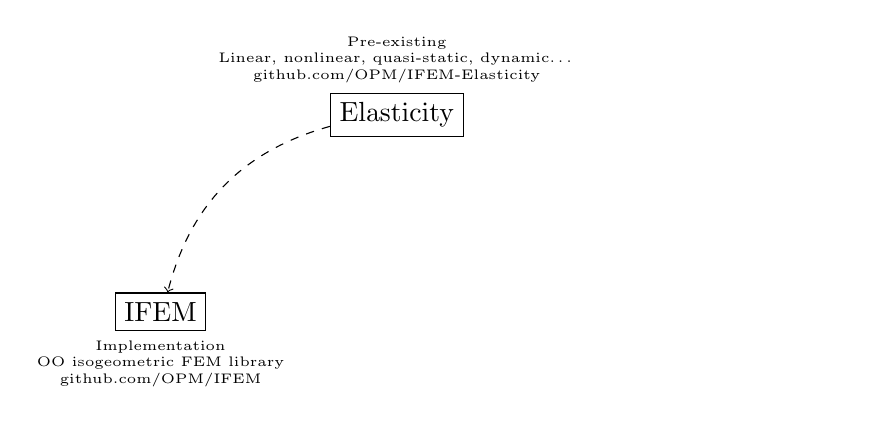
\begin{tikzpicture}
      \node[draw] (ifem) at (0,0) {IFEM};
      \node[draw] (elasto) at (3,2.5) {Elasticity};
      \node[draw,white] (poro) at (4,0) {Poroelasticity};
      \node[draw,white] (frac) at (7,2.5) {Fracture};
      \draw[->,dashed] (elasto) edge[bend right] (ifem);
      \node[below=0 of ifem, align=center]
      {\tiny Implementation \\[-0.6em]
        \tiny OO isogeometric FEM library \\[-0.6em]
        \tiny github.com/OPM/IFEM};
      \node[above=0 of elasto, align=center]
      {\tiny Pre-existing \\[-0.6em]
        \tiny Linear, nonlinear, quasi-static, dynamic\ldots \\[-0.6em]
        \tiny github.com/OPM/IFEM-Elasticity};
      \node[below=0 of poro, align=center, white]
      {\tiny New, Biot model (Darcy flow) \\[-0.6em]
        \tiny Mixed and equal order \\[-0.6em]
        \tiny github.com/OPM/IFEM-PoroElasticity};
      \node[above=0 of frac, align=center, white]
      {\tiny New, phase field model \\[-0.6em]
        \tiny Cahn-Hilliard equation \\[-0.6em]
        \tiny github.com/OPM/IFEM-OpenFrac};
    \end{tikzpicture}
  \end{center}
\end{frame}

\begin{frame}
  \frametitle{Overview}
  \begin{center}
    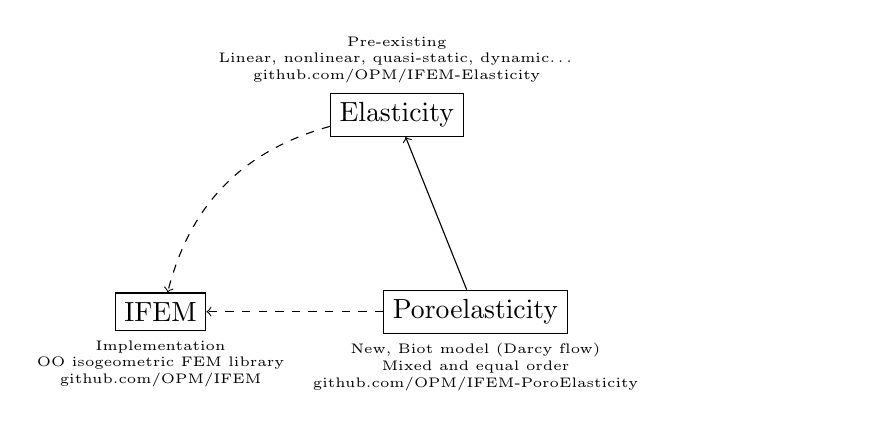
\begin{tikzpicture}
      \node[draw] (ifem) at (0,0) {IFEM};
      \node[draw] (elasto) at (3,2.5) {Elasticity};
      \node[draw] (poro) at (4,0) {Poroelasticity};
      \node[draw,white] (frac) at (7,2.5) {Fracture};
      \draw[->,dashed] (elasto) edge[bend right] (ifem);
      \draw[->] (poro) edge (elasto);
      \draw[->,dashed] (poro) edge (ifem);
      \node[below=0 of ifem, align=center]
      {\tiny Implementation \\[-0.6em]
        \tiny OO isogeometric FEM library \\[-0.6em]
        \tiny github.com/OPM/IFEM};
      \node[above=0 of elasto, align=center]
      {\tiny Pre-existing \\[-0.6em]
        \tiny Linear, nonlinear, quasi-static, dynamic\ldots \\[-0.6em]
        \tiny github.com/OPM/IFEM-Elasticity};
      \node[below=0 of poro, align=center]
      {\tiny New, Biot model (Darcy flow) \\[-0.6em]
        \tiny Mixed and equal order \\[-0.6em]
        \tiny github.com/OPM/IFEM-PoroElasticity};
      \node[above=0 of frac, align=center, white]
      {\tiny New, phase field model \\[-0.6em]
        \tiny Cahn-Hilliard equation \\[-0.6em]
        \tiny github.com/OPM/IFEM-OpenFrac};
    \end{tikzpicture}
  \end{center}
\end{frame}

\begin{frame}
  \frametitle{Overview}
  \begin{center}
    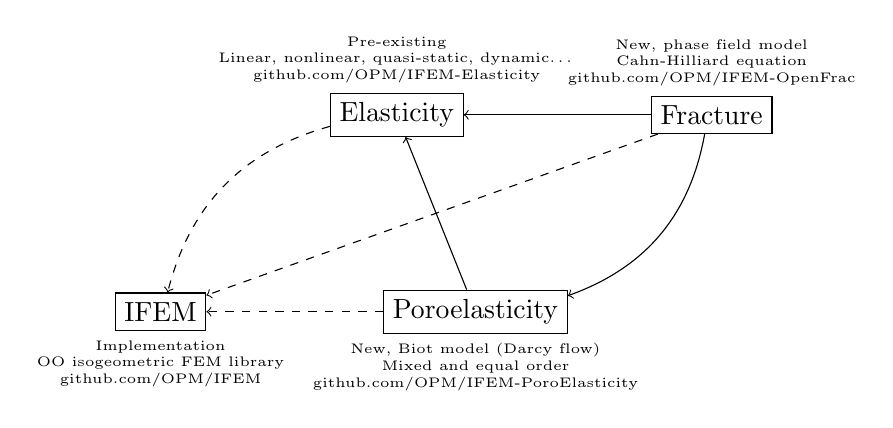
\begin{tikzpicture}
      \node[draw] (ifem) at (0,0) {IFEM};
      \node[draw] (elasto) at (3,2.5) {Elasticity};
      \node[draw] (poro) at (4,0) {Poroelasticity};
      \node[draw] (frac) at (7,2.5) {Fracture};
      \draw[->,dashed] (elasto) edge[bend right] (ifem);
      \draw[->] (poro) edge (elasto);
      \draw[->,dashed] (poro) edge (ifem);
      \draw[->] (frac) edge[bend left] (poro);
      \draw[->] (frac) edge (elasto);
      \draw[->,dashed] (frac) edge (ifem);
      \node[below=0 of ifem, align=center]
      {\tiny Implementation \\[-0.6em]
        \tiny OO isogeometric FEM library \\[-0.6em]
        \tiny github.com/OPM/IFEM};
      \node[above=0 of elasto, align=center]
      {\tiny Pre-existing \\[-0.6em]
        \tiny Linear, nonlinear, quasi-static, dynamic\ldots \\[-0.6em]
        \tiny github.com/OPM/IFEM-Elasticity};
      \node[below=0 of poro, align=center]
      {\tiny New, Biot model (Darcy flow) \\[-0.6em]
        \tiny Mixed and equal order \\[-0.6em]
        \tiny github.com/OPM/IFEM-PoroElasticity};
      \node[above=0 of frac, align=center]
      {\tiny New, phase field model \\[-0.6em]
        \tiny Cahn-Hilliard equation \\[-0.6em]
        \tiny github.com/OPM/IFEM-OpenFrac};
    \end{tikzpicture}
  \end{center}
\end{frame}

\section{Poroelasticity}

\begin{frame}
  \frametitle{Poroelasticity}

  Models flow and deformation in porous media by coupling (linear) elasticity
  with Darcy flow. \\~\\
  
  The equilibrium equation:
  \[
    \nabla \cdot \underbrace{\left(\bm{\sigma}' - \alpha p \bm{I} \right)}_{\text{total stress}} + \bm{F} = 0
  \]
  We use a linear stress-strain relationship with small displacements.
  \[
    \bm{\sigma}' = \bm{D} :
    \underbrace{\frac{1}{2}\left( \nabla \bm{u} + \nabla \bm{u}^\intercal \right)}_{\text{strain}}
  \]
\end{frame}

\begin{frame}
  \frametitle{Poroelasticity}

  Change of fluid content:
  \[
    \frac{\fdd}{\fdd t}\left( \frac{p}{M} + \alpha \nabla \cdot \bm{u} \right) =
    - \nabla \cdot \bm{v}_f + s
  \]
  Darcy's law:
  \[
    \bm{v}_f = -\bm{\kappa}(\nabla p - \rho_f \bm{g})
  \]
  Here, $\alpha$ is \emph{Biot's coefficient} and $M$ can be termed \emph{Biot's
  modulus} (or if you prefer, $\nicefrac{1}{M}$ is the
  \emph{constrained specific storage coefficient}.)
\end{frame}

\begin{frame}
  \frametitle{Poroelasticity}

  The model in final form (and Voigt notation):
  \begin{align*}
    \bm{L}^\intercal \bm{CLu} - \alpha \bm{L}^\intercal \bm{m} p + \bm{F} &= 0 \\
    \alpha \nabla \cdot \dot{\bm{u}} + \frac{1}{M}\dot{p}
    - \nabla \cdot \bm{\kappa}(\nabla p - \rho_f\bm{g}) - s &= 0
  \end{align*}
  Here, $\bm{m}$ and $\bm{L}$ are the Voigt notation identity matrix and
  differential operator.
  \[
    \bm{m} = \begin{pmatrix} 1 \\ 1 \\ 1 \\ 0 \\ 0 \\ 0 \end{pmatrix} \qquad
    \bm{L} = \begin{pmatrix}
      \partial_x & & \\
      & \partial_y & \\
      & & \partial_z \\
      & \partial_z & \partial_y \\
      \partial_z & & \partial_x \\
      \partial_y & \partial_x &
    \end{pmatrix}
  \]
\end{frame}

\section{Finite element discretization}

\begin{frame}
  \frametitle{Finite element discretization}

  \[
    \begin{pmatrix} & \\ \bm{Q}^\intercal & \bm{S} \end{pmatrix}
    \begin{pmatrix} \dot{\bm{u}} \\ \dot{\bm{p}} \end{pmatrix} +
    \begin{pmatrix} \bm{K} & -\bm{Q} \\ & \bm{H} \end{pmatrix}
    \begin{pmatrix} \bm{u} \\ \bm{p} \end{pmatrix} =
    \begin{pmatrix} \bm{f}_u \\ \bm{f}_p \end{pmatrix}
  \]
  Where
  \begin{align*}
    \bm{K} &= \int_\Omega \bm{B}^\intercal \bm{CB} \qquad
             & \bm{B} &= \bm{L} \bm{N}_u \\
    \bm{Q} &= \int_\Omega \bm{B}^\intercal \alpha \bm{m} \bm{N}_u \qquad
             & \bm{f}_u &= \int_\Omega \bm{N}_u^\intercal \bm{F}
                          + \int_{\Gamma_t} \bm{N}_u^\intercal \bm{t} \\
    \bm{H} &= \int_\Omega \nabla \bm{N}_p^\intercal \bm{\kappa} \nabla \bm{N}_p \qquad
             & \bm{f}_p &= \int_\Omega \nabla \bm{N}_p^\intercal \bm{\kappa} \rho_f \bm{g}
                          + \int_\Omega \bm{N}_p^\intercal s
                          - \int_{\Gamma_q} \bm{N}_p^\intercal \bm{q} \\
    \bm{S} &= \int_\Omega \bm{N}_p^\intercal \frac{1}{M} \bm{N}_p
  \end{align*}
\end{frame}

\section{Dynamic formulation}

\begin{frame}
  \frametitle{Dynamic formulation}

  The equilibrium equation
  \[
    \nabla \cdot \left(\bm{\sigma}' - \alpha p \bm{I} \right) + \bm{F} = 0
  \]
  provides a quasi-static model, which is assumed to be in static equilibrium at
  all times. (The time dependency comes via coupling.) \\~\\

  We will generally prefer the dynamic formulation, which
  \[
    - \rho_\text{s} \ddot{\bm u} +  \nabla \left(\bm{\sigma}' - \alpha p \bm{I} \right) + \bm{F} = 0
  \]
\end{frame}

\begin{frame}
  \frametitle{Dynamic formulation}

  The matrix form then becomes
  \[
    \begin{pmatrix} \bm{M} & \\ & \end{pmatrix}
    \begin{pmatrix} \ddot{\bm{u}} \\ \ddot{\bm{p}} \end{pmatrix} +
    \begin{pmatrix} & \\ \bm{Q}^\intercal & \bm{S} \end{pmatrix}
    \begin{pmatrix} \dot{\bm{u}} \\ \dot{\bm{p}} \end{pmatrix} +
    \begin{pmatrix} \bm{K} & -\bm{Q} \\ & \bm{H} \end{pmatrix}
    \begin{pmatrix} \bm{u} \\ \bm{p} \end{pmatrix} =
    \begin{pmatrix} \bm{f}_u \\ \bm{f}_p \end{pmatrix}
  \]
  In these cases, we use a predictor-corrector Newmark method for timestepping,
  which solves simultaneously for accelerations $\bm a$, velocities $\bm v$ and
  primary unknowns $\bm d$ by substituting the \emph{Newmark formulas}
  \begin{align*}
    \bm d^{n+1} &= \bm d^n + \Delta t \bm v^n +
    \frac{(\Delta t)^2}{2} \left( (1-2\beta)\bm a^n + 2\beta\bm a^{n+1} \right) \\
    \bm v^{n+1} &= \bm v^n + \Delta t \left( (1-\gamma)\bm a^n + \gamma \bm a^{n+1} \right)
  \end{align*}
  In the quasi-static case, backwards Euler is sufficient.
\end{frame}

\section{Novelty}

\begin{frame}
  \frametitle{Pressure oscillations}

  Traction is applied instantaneously, but the excess pore pressure can take a
  long time to dissipate. In cases with low permeability, this can cause boundary
  layers with rapidly changing pressure, leading to spurious oscillations. \\~\\

  We hope to alleviate this problem using a mixed-order method, where
  displacements have order $n$ and pressure order $n-1$. \\~\\

  \textbf{Note}: This is \emph{not} a div-compatible formulation, which is
  expected to help even more. \\~\\
\end{frame}

\section{1D Consolidation}

\begin{frame}
  \frametitle{1D Consolidation (Terzhagi)}

  \begin{center}
    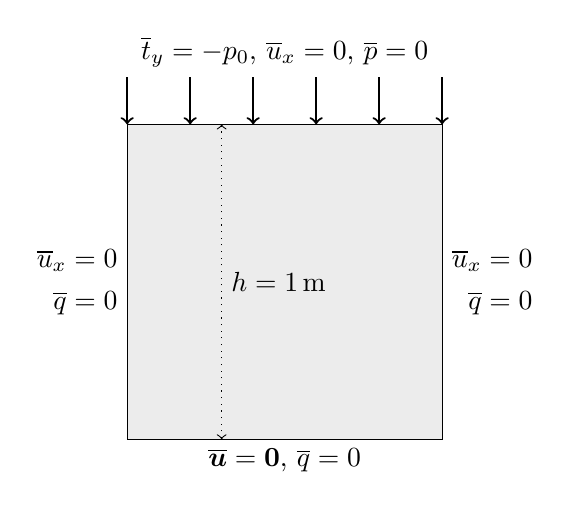
\begin{tikzpicture}[scale=4]
      \filldraw[fill=gray!15, draw=black] (0,0) rectangle (1,1);
      \foreach \x in {0, 0.2, 0.4, 0.6, 0.8, 1}
      \draw[thick, ->] (\x,1.15) -- (\x,1);
      \draw[<->, dotted] (0.3,0) -- (0.3,1);
      \node[anchor=west] at (0.3, 0.5) {$h = \SI{1}{\meter}$};
      \node[anchor=south] at (0.5, 1.15) {
        $\overline{t}_y = -p_0$,
        $\overline{u}_x = 0$,
        $\overline{p} = 0$
      };
      \node[anchor=north] at (0.5, 0.0) {
        $\overline{\bm u} = \bm 0$,
        $\overline{q} = 0$
      };
      \node[anchor=west] at (1.0, 0.5) {
        $\begin{aligned}
          \overline{u}_x &= 0 \\
          \overline{q} &= 0
        \end{aligned}$
      };
      \node[anchor=east] at (0.0, 0.5) {
        $\begin{aligned}
          \overline{u}_x &= 0 \\
          \overline{q} &= 0
        \end{aligned}$
      };
    \end{tikzpicture}
  \end{center}
\end{frame}

\begin{frame}
  \frametitle{Convergence study}

  \begin{align*}
    E &= \SI{0.67}{\pascal} \qquad & \nu &= 0.25 \\
    k &= \SI{1}{\meter\per\second} \qquad & p_0 &= \SI{1}{\pascal}
  \end{align*}

  Analytical solution:
  \[
    \frac{p}{p_0} = \frac{4}{\pi}
    \sum_{i=1}^\infty \frac{(-1)^{i-1}}{2i-1}
    \cos\left[ (2i-1) \frac{\pi y}{2 h} \right]
    \exp\left[ -(2i-1)^2 \frac{\pi^2 c_v t}{4h^2} \right]
  \]
  where $c_v$ is the consolidation coefficient
  \[
    c_v = \kappa \left( \frac{1}{M} + \frac{\alpha^2}{K + \frac{4}{3}G} \right)^{-1}
  \]
\end{frame}

\begin{frame}
  \frametitle{Convergence study}

  \begin{center}
    \begin{tikzpicture}
      \begin{axis}[
        xmode=log,
        ymode=log,
        width=0.8\textwidth,
        height=0.6\textwidth,
        xlabel={$N = \sharp$ DOFs},
        ylabel={$\nicefrac{\|p^h - p\|_{L^2}}{\|p\|_{L^2}}$},
        legend style={
          at={(axis description cs:1,0.5)},
          anchor=west,
          font=\scriptsize,
          draw=none,
        },
        legend cell align=left,
        ]
        \addplot[mark=*, thick, magenta]
        table[x index={0}, y index={1}]{data/conv/lin.csv};
        \addplot[mark=none, dashed, magenta]
        table[x index={0}, y index={1}]{data/conv/comp-lin.csv};
        \addplot[mark=*, thick, blue]
        table[x index={0}, y index={1}]{data/conv/quad.csv};
        \addplot[mark=none, dashed, blue]
        table[x index={0}, y index={1}]{data/conv/comp-quad.csv};
        \addplot[mark=*, thick, red]
        table[x index={0}, y index={1}]{data/conv/cub.csv};
        \addplot[mark=none, dashed, red]
        table[x index={0}, y index={1}]{data/conv/comp-cub.csv};
        \legend{
          $p=1$,
          $\mathcal{O}(N^{-1})$,
          $p=2$,
          $\mathcal{O}(N^{-\nicefrac{3}{2}})$,
          $p=3$,
          $\mathcal{O}(N^{-2})$,
        }
      \end{axis}
    \end{tikzpicture}
  \end{center}
\end{frame}

\begin{frame}
  \frametitle{Low permeability}

  \begin{align*}
    E &= \SI{6}{\giga\pascal} \qquad & \nu &= 0.4 \\
    k &= \SI{1.962e-14}{\meter\per\second} \qquad & p_0 &= \SI{1}{\mega\pascal} \\
    h &= \SI{8}{\milli\meter}
  \end{align*}

  This case has more realistic material parameters, including a very low
  permeability. We should expect to see pressure oscillations for very small
  $t$.
\end{frame}

\begin{frame}
  \frametitle{Low permeability ($\Delta t = \Delta t_\text{c}$)}

  \begin{center}
    \begin{tikzpicture}
      \begin{axis}[
        xmin=0, xmax=0.0085,
        ymin=0, ymax=1.15,
        width=0.8\textwidth,
        height=0.5\textwidth,
        xtick={0,0.008},
        xticklabels={$0$,$1$},
        minor xtick=data,
        ytick={0,1},
        scaled ticks=false,
        axis lines=left,
        xlabel={$\nicefrac{y}{h}$},
        ylabel={$\nicefrac{p}{p_0}$},
        xlabel style={at={(axis description cs:0.5,0)}},
        ylabel style={rotate=-90, at={(axis description cs:0,0.5)}},
        legend style={
          at={(axis description cs:1,0.5)},
          anchor=west,
          font=\scriptsize,
          draw=none,
        },
        legend cell align=left,
        ]
        \addplot[draw=none]
        table[x index={0}, y index={1}]{data/terzhagi-crit/ticks.csv};
        \addplot[mark=none, thick, blue]
        table[x index={0}, y index={1}]{data/terzhagi-crit/data-0.csv};
        \addplot[mark=none, thick, red]
        table[x index={0}, y index={1}]{data/terzhagi-crit/data-1.csv};
        \addplot[mark=none, thick, green!50!black]
        table[x index={0}, y index={1}]{data/terzhagi-crit/data-2.csv};
        \addplot[mark=none, thick, cyan]
        table[x index={0}, y index={1}]{data/terzhagi-crit/data-3.csv};
        \addplot[mark=none, thick, purple]
        table[x index={0}, y index={1}]{data/terzhagi-crit/data-4.csv};
        \legend{
          $t=2\Delta t_\text{c}$,
          $t=100\Delta t_\text{c}$,
          $t=500\Delta t_\text{c}$,
          $t=2000\Delta t_\text{c}$,
          $t=5000\Delta t_\text{c}$,
        }
      \end{axis}
    \end{tikzpicture}
  \end{center}
\end{frame}

\begin{frame}
  \frametitle{Low permeability ($\Delta t = 0.1 \Delta t_\text{c}$)}

  \begin{center}
    \begin{tikzpicture}
      \begin{axis}[
        xmin=0, xmax=0.0085,
        ymin=0, ymax=1.15,
        width=0.8\textwidth,
        height=0.5\textwidth,
        xtick={0,0.008},
        xticklabels={$0$,$1$},
        minor xtick=data,
        ytick={0,1},
        scaled ticks=false,
        axis lines=left,
        xlabel={$\nicefrac{y}{h}$},
        ylabel={$\nicefrac{p}{p_0}$},
        xlabel style={at={(axis description cs:0.5,0)}},
        ylabel style={rotate=-90, at={(axis description cs:0,0.5)}},
        legend style={
          at={(axis description cs:1,0.5)},
          anchor=west,
          font=\scriptsize,
          draw=none,
        },
        legend cell align=left,
        ]
        \addplot[draw=none]
        table[x index={0}, y index={1}]{data/terzhagi-subcrit/ticks.csv};
        \addplot[mark=none, thick, magenta]
        table[x index={0}, y index={1}]{data/terzhagi-subcrit/data-0.csv};
        \addplot[mark=none, thick, blue]
        table[x index={0}, y index={1}]{data/terzhagi-subcrit/data-1.csv};
        \addplot[mark=none, thick, red]
        table[x index={0}, y index={1}]{data/terzhagi-subcrit/data-2.csv};
        \addplot[mark=none, thick, green!50!black]
        table[x index={0}, y index={1}]{data/terzhagi-subcrit/data-3.csv};
        \addplot[mark=none, thick, cyan]
        table[x index={0}, y index={1}]{data/terzhagi-subcrit/data-4.csv};
        \addplot[mark=none, thick, purple]
        table[x index={0}, y index={1}]{data/terzhagi-subcrit/data-5.csv};
        \legend{
          $t=0.1\Delta t_\text{c}$,
          $t=2\Delta t_\text{c}$,
          $t=100\Delta t_\text{c}$,
          $t=500\Delta t_\text{c}$,
          $t=2000\Delta t_\text{c}$,
          $t=5000\Delta t_\text{c}$,
        }
      \end{axis}
    \end{tikzpicture}
  \end{center}
\end{frame}

% \section{2D consolidation}

% \begin{frame}
%   \frametitle{2D consolidation}
%   \begin{center}
%     \begin{tikzpicture}[scale=0.7]
%       \filldraw[fill=gray!15, draw=black] (0,0) rectangle (8,5);
%       \foreach \x in {0, 0.5, 1}
%       \draw[thick, ->] (\x,5.75) -- (\x,5);
%       \draw[<->, dotted] (1,0) -- (1,5);
%       \node[anchor=west] at (1, 3) {$h = \SI{5}{\meter}$};
%       \draw[<->, dotted] (0,1) -- (8,1);
%       \node[anchor=south] at (5, 1) {$w = \SI{8}{\meter}$};
%       \node[anchor=south] at (0.5, 5.75) {
%         $\overline{t}_y = -p_0$
%       };
%       \node[anchor=south] at (4, 5) {
%         $p = 0$
%       };
%       \node[anchor=north] at (4, 0.0) {
%         $\overline{\bm u} = \bm 0$,
%         $\overline{q} = 0$
%       };
%       \node[anchor=east] at (0, 2.5) {
%         $\begin{aligned}
%           \overline{u}_x &= 0 \\
%           \overline{q} &= 0
%         \end{aligned}$
%       };
%       \node[anchor=west] at (8, 2.5) {
%         $\begin{aligned}
%           \overline{u}_x &= 0 \\
%           \overline{q} &= 0
%         \end{aligned}$
%       };
%     \end{tikzpicture}
%   \end{center}
%   Implemented as a multipatch model with a $C^0$-continuous internal boundary at
%   $x=1$.
% \end{frame}

% \begin{frame}
%   \frametitle{2D consolidation}

%   Pressure distribution at $t = \SI{4}{\second}$.
%   \begin{center}
%     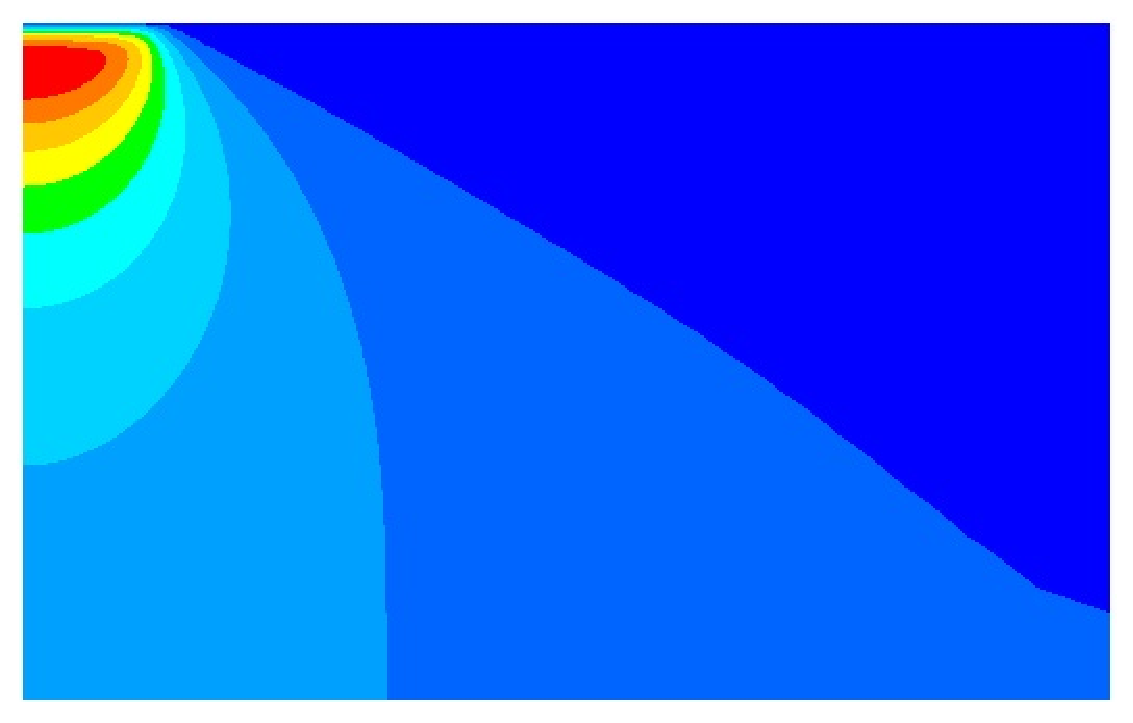
\includegraphics[height=6cm]{figs/OGS2DExcessPorePrDist}
%   \end{center}
% \end{frame}

% \begin{frame}
%   \frametitle{2D consolidation}

%   Pressure distribution at $t = \SI{4}{\second}$, left edge.
%   \begin{center}
%     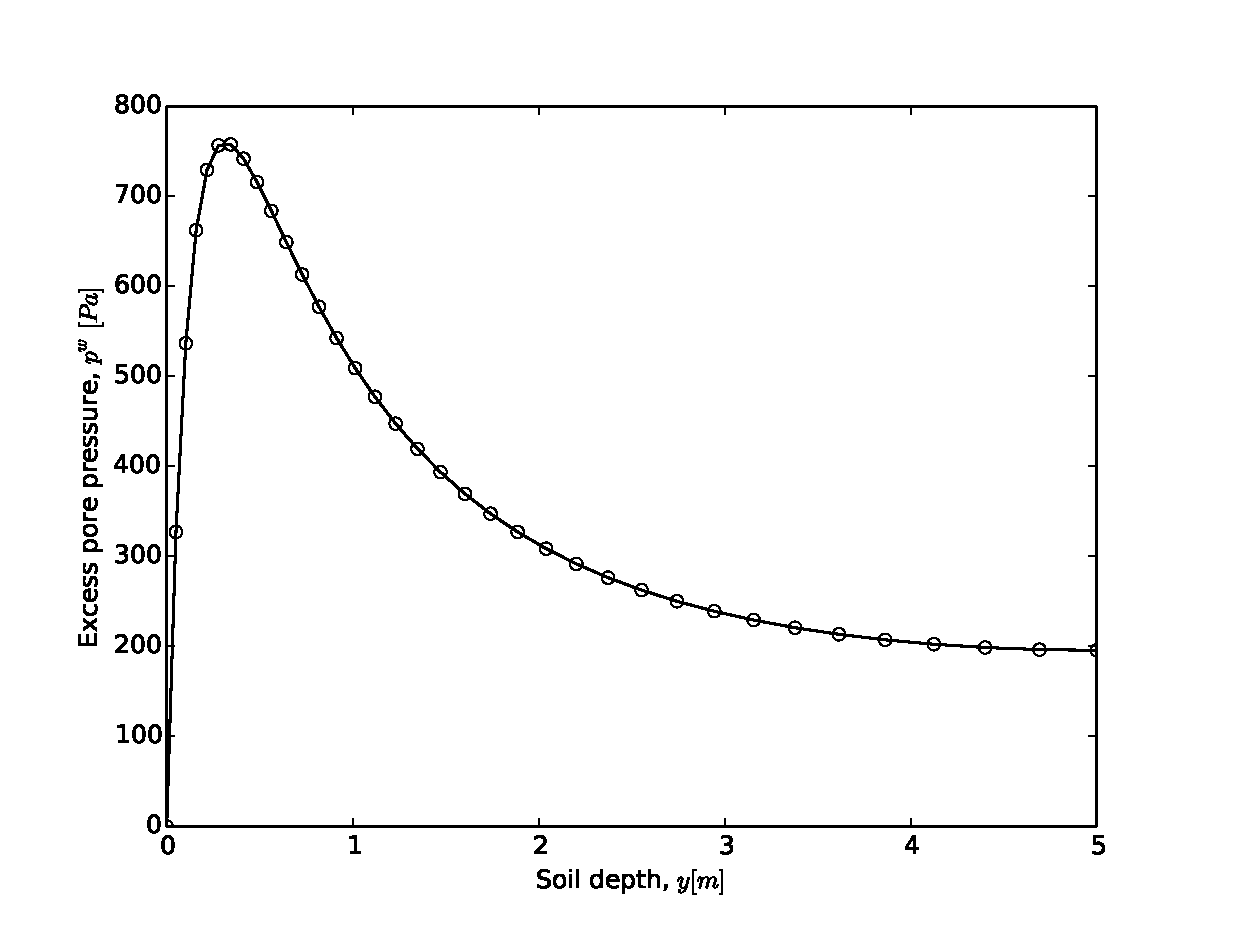
\includegraphics[height=6cm]{figs/OGS2DExcessPorePrProf}
%   \end{center}
% \end{frame}

\section{Pressure oscillations}

\begin{frame}
  \frametitle{Pressure oscillations}

  Case due to Joachim Berdal Haga.
  \begin{center}
    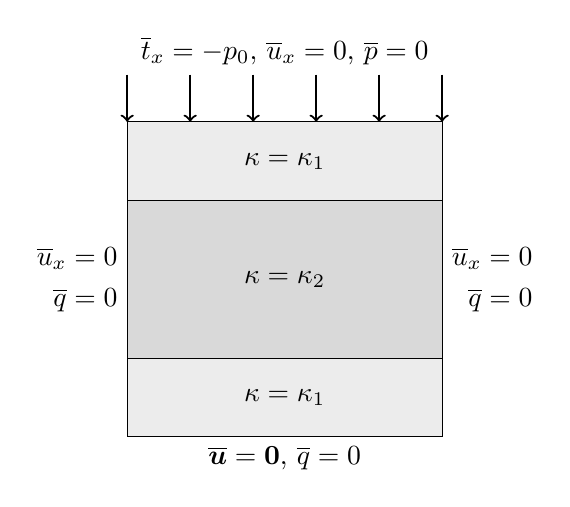
\begin{tikzpicture}[scale=4]
      \filldraw[fill=gray!15, draw=black] (0,0) rectangle (1,0.25);
      \filldraw[fill=gray!30, draw=black] (0,0.25) rectangle (1,0.75);
      \filldraw[fill=gray!15, draw=black] (0,0.75) rectangle (1,1);
      \foreach \x in {0, 0.2, 0.4, 0.6, 0.8, 1}
      \draw[thick, ->] (\x,1.15) -- (\x,1);
      \node at (0.5, 0.5) {$\kappa = \kappa_2$};
      \node at (0.5, 0.125) {$\kappa = \kappa_1$};
      \node at (0.5, 0.875) {$\kappa = \kappa_1$};
      \node[anchor=south] at (0.5, 1.15) {
        $\overline{t}_x = -p_0$,
        $\overline{u}_x = 0$,
        $\overline{p} = 0$
      };
      \node[anchor=north] at (0.5, 0.0) {
        $\overline{\bm u} = \bm 0$,
        $\overline{q} = 0$
      };
      \node[anchor=west] at (1.0, 0.5) {
        $\begin{aligned}
          \overline{u}_x &= 0 \\
          \overline{q} &= 0
        \end{aligned}$
      };
      \node[anchor=east] at (0.0, 0.5) {
        $\begin{aligned}
          \overline{u}_x &= 0 \\
          \overline{q} &= 0
        \end{aligned}$
      };
    \end{tikzpicture}
  \end{center}
\end{frame}

\begin{frame}
  \frametitle{Pressure oscillations}

  \begin{align*}
    E &= \SI{0.67}{\giga\pascal} \qquad & \nu &= 0.25 \\
    \kappa_1 &= \SI{1}{\meter^2\per\pascal\second} \qquad & p_0 &= \SI{1}{\pascal} \\
    \kappa_2 &= \SI{1e-8}{\meter^2\per\pascal\second} \qquad & h &= \SI{8}{\milli\meter}
  \end{align*}
\end{frame}

\begin{frame}
  \frametitle{Pressure oscillations}

  $N=60$, uniform, equal order, full continuity.
  \begin{center}
    \begin{tikzpicture}
      \begin{axis}[
        xmin=0.15, xmax=0.85,
        ymin=0, ymax=2,
        width=0.95\textwidth,
        height=0.5\textwidth,
        xtick={0.25,0.5,0.75},
        minor xtick=data,
        ytick={0,1,2},
        scaled ticks=false,
        axis lines=left,
        xlabel style={at={(axis description cs:0.75,0)}},
        ylabel style={rotate=-90, at={(axis description cs:0,0.75)}},
        ]
        \addplot[draw=none]
        table[x index={0}, y index={1}]{data/haga-unif-max-equal/ticks.csv};
        \addplot[mark=none, thick, blue]
        table[x index={0}, y index={1}]{data/haga-unif-max-equal/data-1.csv};
        \addplot[mark=none, thick, red]
        table[x index={0}, y index={1}]{data/haga-unif-max-equal/data-2.csv};
        \addplot[mark=none, thick, green!50!black]
        table[x index={0}, y index={1}]{data/haga-unif-max-equal/data-3.csv};
        \addplot[mark=none, thick, cyan]
        table[x index={0}, y index={1}]{data/haga-unif-max-equal/data-4.csv};
      \end{axis}
    \end{tikzpicture}
  \end{center}
\end{frame}

\begin{frame}
  \frametitle{Pressure oscillations}

  $N=60$, uniform, mixed order, full continuity.
  \begin{center}
    \begin{tikzpicture}
      \begin{axis}[
        xmin=0.15, xmax=0.85,
        ymin=0, ymax=2,
        width=0.95\textwidth,
        height=0.5\textwidth,
        xtick={0.25,0.5,0.75},
        minor xtick=data,
        ytick={0,1,2},
        scaled ticks=false,
        axis lines=left,
        xlabel style={at={(axis description cs:0.75,0)}},
        ylabel style={rotate=-90, at={(axis description cs:0,0.75)}},
        ]
        \addplot[draw=none]
        table[x index={0}, y index={1}]{data/haga-unif-max-mixed/ticks.csv};
        \addplot[mark=none, thick, blue]
        table[x index={0}, y index={1}]{data/haga-unif-max-mixed/data-1.csv};
        \addplot[mark=none, thick, red]
        table[x index={0}, y index={1}]{data/haga-unif-max-mixed/data-2.csv};
        \addplot[mark=none, thick, green!50!black]
        table[x index={0}, y index={1}]{data/haga-unif-max-mixed/data-3.csv};
        \addplot[mark=none, thick, cyan]
        table[x index={0}, y index={1}]{data/haga-unif-max-mixed/data-4.csv};
      \end{axis}
    \end{tikzpicture}
  \end{center}
\end{frame}

\begin{frame}
  \frametitle{Pressure oscillations}

  $N=60$, uniform, equal order, full continuity.
  \begin{center}
    \begin{tikzpicture}
      \begin{axis}[
        xmin=0.15, xmax=0.85,
        ymin=0, ymax=2,
        width=0.95\textwidth,
        height=0.5\textwidth,
        xtick={0.25,0.5,0.75},
        minor xtick=data,
        ytick={0,1,2},
        scaled ticks=false,
        axis lines=left,
        xlabel style={at={(axis description cs:0.75,0)}},
        ylabel style={rotate=-90, at={(axis description cs:0,0.75)}},
        ]
        \addplot[draw=none]
        table[x index={0}, y index={1}]{data/haga-unif-min-equal/ticks.csv};
        \addplot[mark=none, thick, blue]
        table[x index={0}, y index={1}]{data/haga-unif-min-equal/data-1.csv};
        \addplot[mark=none, thick, red]
        table[x index={0}, y index={1}]{data/haga-unif-min-equal/data-2.csv};
        \addplot[mark=none, thick, green!50!black]
        table[x index={0}, y index={1}]{data/haga-unif-min-equal/data-3.csv};
        \addplot[mark=none, thick, cyan]
        table[x index={0}, y index={1}]{data/haga-unif-min-equal/data-4.csv};
      \end{axis}
    \end{tikzpicture}
  \end{center}
\end{frame}

\begin{frame}
  \frametitle{Pressure oscillations}

  $N=60$, uniform, mixed order, minimal continuity.
  \begin{center}
    \begin{tikzpicture}
      \begin{axis}[
        xmin=0.15, xmax=0.85,
        ymin=0, ymax=2,
        width=0.95\textwidth,
        height=0.5\textwidth,
        xtick={0.25,0.5,0.75},
        minor xtick=data,
        ytick={0,1,2},
        scaled ticks=false,
        axis lines=left,
        xlabel style={at={(axis description cs:0.75,0)}},
        ylabel style={rotate=-90, at={(axis description cs:0,0.75)}},
        ]
        \addplot[draw=none]
        table[x index={0}, y index={1}]{data/haga-unif-min-mixed/ticks.csv};
        \addplot[mark=none, thick, blue]
        table[x index={0}, y index={1}]{data/haga-unif-min-mixed/data-1.csv};
        \addplot[mark=none, thick, red]
        table[x index={0}, y index={1}]{data/haga-unif-min-mixed/data-2.csv};
        \addplot[mark=none, thick, green!50!black]
        table[x index={0}, y index={1}]{data/haga-unif-min-mixed/data-3.csv};
        \addplot[mark=none, thick, cyan]
        table[x index={0}, y index={1}]{data/haga-unif-min-mixed/data-4.csv};
      \end{axis}
    \end{tikzpicture}
  \end{center}
\end{frame}

\begin{frame}
  \frametitle{Pressure oscillations}

  Graded mesh, equal order, full continuity.
  \begin{center}
    \begin{tikzpicture}
      \begin{axis}[
        xmin=0.15, xmax=0.85,
        ymin=0, ymax=2,
        width=0.95\textwidth,
        height=0.5\textwidth,
        xtick={0.25,0.5,0.75},
        minor xtick=data,
        ytick={0,1,2},
        scaled ticks=false,
        axis lines=left,
        xlabel style={at={(axis description cs:0.75,0)}},
        ylabel style={rotate=-90, at={(axis description cs:0,0.75)}},
        ]
        \addplot[draw=none]
        table[x index={0}, y index={1}]{data/haga-grad-max-equal/ticks.csv};
        \addplot[mark=none, thick, blue]
        table[x index={0}, y index={1}]{data/haga-grad-max-equal/data-1.csv};
        \addplot[mark=none, thick, red]
        table[x index={0}, y index={1}]{data/haga-grad-max-equal/data-2.csv};
        \addplot[mark=none, thick, green!50!black]
        table[x index={0}, y index={1}]{data/haga-grad-max-equal/data-3.csv};
        \addplot[mark=none, thick, cyan]
        table[x index={0}, y index={1}]{data/haga-grad-max-equal/data-4.csv};
      \end{axis}
    \end{tikzpicture}
  \end{center}
\end{frame}

\begin{frame}
  \frametitle{Pressure oscillations}

  Graded mesh, mixed order, full continuity.
  \begin{center}
    \begin{tikzpicture}
      \begin{axis}[
        xmin=0.15, xmax=0.85,
        ymin=0, ymax=2,
        width=0.95\textwidth,
        height=0.5\textwidth,
        xtick={0.25,0.5,0.75},
        minor xtick=data,
        ytick={0,1,2},
        scaled ticks=false,
        axis lines=left,
        xlabel style={at={(axis description cs:0.75,0)}},
        ylabel style={rotate=-90, at={(axis description cs:0,0.75)}},
        ]
        \addplot[draw=none]
        table[x index={0}, y index={1}]{data/haga-grad-max-mixed/ticks.csv};
        \addplot[mark=none, thick, blue]
        table[x index={0}, y index={1}]{data/haga-grad-max-mixed/data-1.csv};
        \addplot[mark=none, thick, red]
        table[x index={0}, y index={1}]{data/haga-grad-max-mixed/data-2.csv};
        \addplot[mark=none, thick, green!50!black]
        table[x index={0}, y index={1}]{data/haga-grad-max-mixed/data-3.csv};
        \addplot[mark=none, thick, cyan]
        table[x index={0}, y index={1}]{data/haga-grad-max-mixed/data-4.csv};
      \end{axis}
    \end{tikzpicture}
  \end{center}
\end{frame}

\begin{frame}
  \frametitle{Pressure oscillations}

  Graded mesh, equal order, minimal continuity.
  \begin{center}
    \begin{tikzpicture}
      \begin{axis}[
        xmin=0.15, xmax=0.85,
        ymin=0, ymax=2,
        width=0.95\textwidth,
        height=0.5\textwidth,
        xtick={0.25,0.5,0.75},
        minor xtick=data,
        ytick={0,1,2},
        scaled ticks=false,
        axis lines=left,
        xlabel style={at={(axis description cs:0.75,0)}},
        ylabel style={rotate=-90, at={(axis description cs:0,0.75)}},
        ]
        \addplot[draw=none]
        table[x index={0}, y index={1}]{data/haga-grad-min-equal/ticks.csv};
        \addplot[mark=none, thick, blue]
        table[x index={0}, y index={1}]{data/haga-grad-min-equal/data-1.csv};
        \addplot[mark=none, thick, red]
        table[x index={0}, y index={1}]{data/haga-grad-min-equal/data-2.csv};
        \addplot[mark=none, thick, green!50!black]
        table[x index={0}, y index={1}]{data/haga-grad-min-equal/data-3.csv};
        \addplot[mark=none, thick, cyan]
        table[x index={0}, y index={1}]{data/haga-grad-min-equal/data-4.csv};
      \end{axis}
    \end{tikzpicture}
  \end{center}
\end{frame}

\begin{frame}
  \frametitle{Pressure oscillations}

  Graded mesh, mixed order, minimal continuity.
  \begin{center}
    \begin{tikzpicture}
      \begin{axis}[
        xmin=0.15, xmax=0.85,
        ymin=0, ymax=2,
        width=0.95\textwidth,
        height=0.5\textwidth,
        xtick={0.25,0.5,0.75},
        minor xtick=data,
        ytick={0,1,2},
        scaled ticks=false,
        axis lines=left,
        xlabel style={at={(axis description cs:0.75,0)}},
        ylabel style={rotate=-90, at={(axis description cs:0,0.75)}},
        ]
        \addplot[draw=none]
        table[x index={0}, y index={1}]{data/haga-grad-min-mixed/ticks.csv};
        \addplot[mark=none, thick, blue]
        table[x index={0}, y index={1}]{data/haga-grad-min-mixed/data-1.csv};
        \addplot[mark=none, thick, red]
        table[x index={0}, y index={1}]{data/haga-grad-min-mixed/data-2.csv};
        \addplot[mark=none, thick, green!50!black]
        table[x index={0}, y index={1}]{data/haga-grad-min-mixed/data-3.csv};
        \addplot[mark=none, thick, cyan]
        table[x index={0}, y index={1}]{data/haga-grad-min-mixed/data-4.csv};
      \end{axis}
    \end{tikzpicture}
  \end{center}
\end{frame}

\section{Fracturing}

\begin{frame}
  \frametitle{Fracturing}

  Fractures in the material are handled with a phase field formulation: a
  function $c(\bm x)$, $0 \leq c \leq 1$, where $c=1$ indicates unbroken
  material and $c=0$ indicates fully broken material. It satisfies the
  \emph{Cahn-Hilliard} equation (here second order):
  \[
    \frac{2 \ell_0}{\mathcal{G}_\text{c}} g'(c) \mathcal{H}
    + c - 4 \ell_0^2 \nabla^2 c = 1.
  \]
  $\ell_0$ is a spatial smearing parameter which should be on the order of mesh
  size, $\mathcal{G}_\text{c}$ is the fracture energy density, and $g(c)$ is a
  degradation function, for example $g(c) = c^2$ (making the CH-equation linear).
\end{frame}

\begin{frame}
  \frametitle{Fracturing (Miehe, Mauthe)}

  The parameter $\mathcal{H}$ represents one direction of the coupling, and it
  is the driving force of crack formation. It is usually chosen as a measure of
  \emph{tensile} strain energy, e.g.
  \[
    \mathcal{H} = \max \left(
      0, \sum_{a} \left( \frac{\max(0, \sigma^a)}{\sigma_c} \right)^2 - 1
    \right)
  \]
  To prevent an open crack from closing and ``healing'' the material, it is
  necessary to take the maximum over all timesteps.
\end{frame}

\begin{frame}
  \frametitle{Fracturing (Miehe, Mauthe)}

  The coupling in the other direction is realized by replacing the strain energy
  $\psi(\epsilon)$ by the modified form
  \[
    \tilde{\psi}(\epsilon) = g(c) \psi^+(\epsilon) + \psi^-(\epsilon)
  \]
  which uses the degradation function $g(c)$ to suppress the tensile energy in
  damaged areas, while allowing compressive energy everywhere. \\~\\
\end{frame}

\begin{frame}
  \frametitle{Fracturing (Miehe, Mauthe)}

  For poroelasticity, it is also of interest to simulate more complex flow in
  cracks. As a simplification, one may use ordinary Darcy flow with an
  artificially inflated permeability, e.g.
  \[
    |\tilde{\kappa}| \propto \frac{w^2}{12\mu},
  \]
  $\mu$ being the dynamic viscosity of the flud, and
  $w = w(\bm u, \nabla \bm u, c, \nabla c)$ a crack width measure.
\end{frame}

% \begin{frame}
%   \frametitle{Fracturing}

%   The split of the elastic energy makes the elasticity problem nonlinear.
%   However, it is still convex, so relatively simple to solve with an iterative
%   method $\Longrightarrow$ segregated solver. \\~\\

%   However, the coupling can be quite strong. Sometimes you need very many
%   phase/elastic iterations before converging. Literature indicates that a
%   monolithic fully coupled solver can be advantageous. However the complete
%   system is non-convex requiring some creative optimization techniques. (de
%   Lorenzis, Wheeler) \\~\\

%   Here: Single-iteration segregated, with small timesteps when necessary.
% \end{frame}

\begin{frame}
  \frametitle{Pressurized crack}

  Case due to Sneddon.
  \begin{center}
    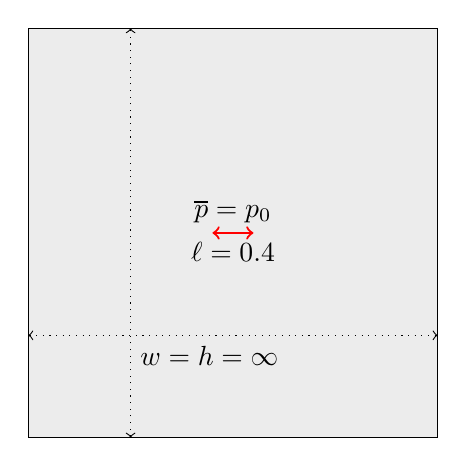
\begin{tikzpicture}[scale=1.3]
      \filldraw[fill=gray!15, draw=black] (0,0) rectangle (4,4);
      \draw[thick, <->, red] (1.8,2) -- (2.2,2);
      \node[anchor=north] at (2,2) {$\ell=0.4$};
      \node[anchor=south] at (2,2) {$\overline{p}=p_0$};
      \draw[<->, dotted] (1,0) -- (1,4);
      \draw[<->, dotted] (0,1) -- (4,1);
      \node[anchor=west] at (1,0.8) {$w = h = \infty$};
    \end{tikzpicture}
  \end{center}
\end{frame}

\begin{frame}
  \frametitle{Pressurized crack}

  \begin{align*}
    E &= \SI{1.0}{\pascal} \qquad & \nu &= 0.2 \\
    \mathcal{G}_\text{c} &= \SI{1}{\newton\per\meter} \qquad & p_0 &= \SI{1}{\milli\pascal} \\
    \alpha &= 0 \qquad & w = h &= \SI{4}{\meter}
  \end{align*}

  Note that $\alpha=0$ yields a completely decoupled formulation, so this is
  strictly elasto-fracture. \\~\\

  Quantity of interest:
  \[
    w(x) = \int_{-\infty}^\infty \nabla c \cdot \bm u \, \text{d} y
  \]
\end{frame}

\begin{frame}
  \frametitle{Pressurized crack}

  $w(x)$ for $N=40, 80, 160$ elements.

  \begin{center}
    \begin{tikzpicture}
      \begin{axis}[
        ymin=0, ymax=0.001,
        width=0.95\textwidth,
        height=0.5\textwidth,
        xtick={1.8, 1.9, 2.0, 2.1, 2.2},
        scaled ticks=false,
        axis lines=left,
        xlabel style={at={(axis description cs:0.75,0)}},
        ylabel style={rotate=-90, at={(axis description cs:0,0.75)}},
        ]
        \addplot[mark=none, thick, green]
        table[x index={0}, y index={1}]{data/sneddon-umr-40.csv};
        \addplot[mark=none, thick, blue]
        table[x index={0}, y index={1}]{data/sneddon-umr-80.csv};
        \addplot[mark=none, thick, red]
        table[x index={0}, y index={1}]{data/sneddon-umr-160.csv};
        % \addplot[mark=none, thick, black, dashed]
        % table[x index={0}, y index={1}]{data/sneddon-exact.csv};
      \end{axis}
    \end{tikzpicture}
  \end{center}
\end{frame}

\section{Finale}

\begin{frame}
  \frametitle{Summary and future work}

  \begin{itemize}
  \item Poroelasticity solver with mixed and equal order methods
  \item The mixed method can keep pressure oscillations localized, unlike the
    equal order method
  \item Basic fracture support implemented
  \end{itemize}

  Future
  \begin{itemize}
  \item Div-compatible spaces
  \item Additional verification of fracture code
  \item Sub-iterative fracture solver
  \item Monolithic fracture solver
  \item More sophisticated flow in cracks
  \end{itemize}
\end{frame}

\begin{frame}
  \begin{center}
    \begin{CJK}{UTF8}{mj}
      \Large 주목해 주셔서 감사합니다
    \end{CJK}
  \end{center}
\end{frame}

\end{document}
